%%%%%%%%%%%%%%%%%%%%%%%%%%%%%%%%%%%%
% Slide options
%%%%%%%%%%%%%%%%%%%%%%%%%%%%%%%%%%%%

% Option 1: Slides with solutions

\documentclass[slidestop,compress,mathserif]{beamer}
\newcommand{\soln}[1]{\textit{#1}}
\newcommand{\solnGr}[1]{#1}

% Option 2: Handouts without solutions

%\documentclass[11pt,containsverbatim,handout]{beamer}
%\usepackage{pgfpages}
%\pgfpagesuselayout{4 on 1}[letterpaper,landscape,border shrink=5mm]
%\newcommand{\soln}[1]{ }
%\newcommand{\solnGr}{ }

%%%%%%%%%%%%%%%%%%%%%%%%%%%%%%%%%%%%
% Style
%%%%%%%%%%%%%%%%%%%%%%%%%%%%%%%%%%%%

\def\chpii@path{../../Chp 2}
\input{../../lec_style.tex}

\usetikzlibrary{overlay-beamer-styles}

%%%%%%%%%%%%%%%%%%%%%%%%%%%%%%%%%%%%
% Preamble
%%%%%%%%%%%%%%%%%%%%%%%%%%%%%%%%%%%%

\title[Lecture 4]{MA 213: Lecture 4}
\subtitle{Module 1: Exploratory Data Analysis and Study Design}
\author{OpenIntro Statistics, 4th Edition}
\institute{$\:$ \\ {\footnotesize Based on slides developed by Mine \c{C}etinkaya-Rundel of OpenIntro. \\
The slides may be copied, edited, and/or shared via the \webLink{http://creativecommons.org/licenses/by-sa/3.0/us/}{CC BY-SA license.} \\
Some images may be included under fair use guidelines (educational purposes).}}
\date{}

%%%%%%%%%%%%%%%%%%%%%%%%%%%%%%%%%%%%
% Begin document
%%%%%%%%%%%%%%%%%%%%%%%%%%%%%%%%%%%%

\begin{document}


%%%%%%%%%%%%%%%%%%%%%%%%%%%%%%%%%%%%
% Title page
%%%%%%%%%%%%%%%%%%%%%%%%%%%%%%%%%%%%

{
\addtocounter{framenumber}{-1} 
{\removepagenumbers 
\usebackgroundtemplate{\includegraphics[width=\paperwidth]{../../OpenIntro_Grid_4_3-01.jpg}}
\begin{frame}

\hfill \includegraphics[width=20mm]{../../oiLogo_highres}

\titlepage

\end{frame}
}
}

%%%%%%%%%%%%%%%%%%%%%%%%%%%%%%%%%%%%
% Sections
%%%%%%%%%%%%%%%%%%%%%%%%%%%%%%%%%%%%


%%%%%%%%%%%%%%%%%%%%%%%%%%%%%%%%%%%%
% Recap/Agenda 
%%%%%%%%%%%%%%%%%%%%%%%%%%%%%%%%%%%%
% TODO better formatting
\begin{frame}
    \frametitle{Module 1: Exploratory Data Analysis and Study Design}
    \begin{itemize}
        \item \hl{Previously: } Examining numerical data (Chapter 2.1)
        \item \hl{This time: } Considering categorial data (Chapter 2.2)
        \item \hl{Reading: } Chapter 2.3 for next time
        \item \hl{Deadlines/Announcements: } 
    \end{itemize}
    
\end{frame}

%%%%%%%%%%%%%%%%%%%%%%%%%%%%%%%%%%%%
% Learning objectives:
%%%%%%%%%%%%%%%%%%%%%%%%%%%%%%%%%%%%
\begin{frame}
    \frametitle{Learning Objectives}
    \begin{itemize}
        \item \textbf{M1, LO1: Classify and Analyze Variables:} Categorize variables based on their types (e.g., numerical/categorical, continuous/discrete, ordinal), assess their association (positive, negative, or independent), and determine which make sense as explanatory vs. response variables.
        \item \textbf{M1, LO3: Use R for Data Management and Exploration:} Utilize R to load, pre-process, and explore data through visualization and summarization techniques.
        \item \textbf{M1, LO4: Visualize and Describe Data Distributions:} Select appropriate visualizations (scatterplots, histograms, box plots, bar plots) to depict data, and describe distributions qualitatively (shape, center, spread, outliers) and quantitatively (mean, median, mode, range, IQR, standard deviation).
    \end{itemize}
\end{frame}


\begin{frame}
\frametitle{Box plot}

The box in a \hl{box plot} represents the middle 50\% of the data, and the thick line in the box is the median.

\begin{center}
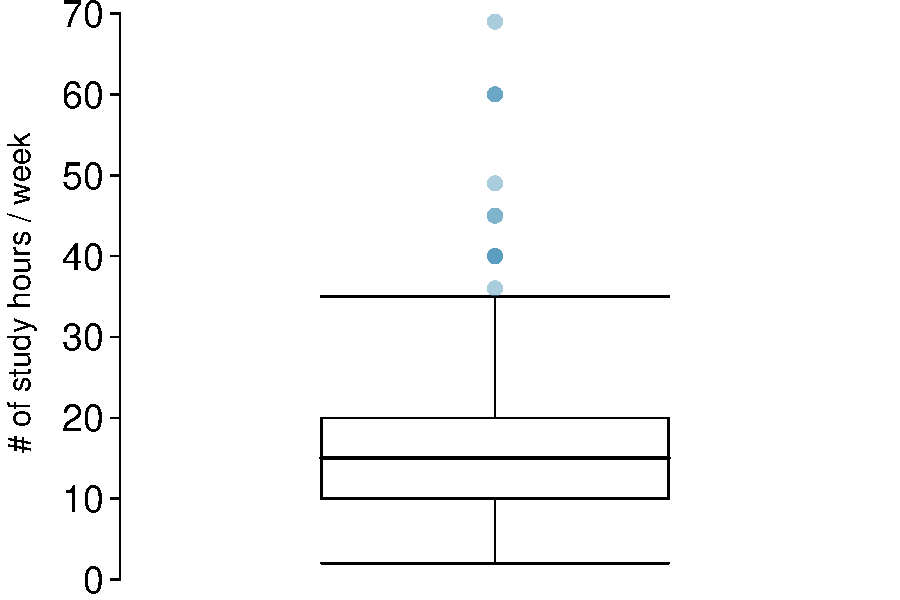
\includegraphics[width=0.7\textwidth]{\chpii@path/2-1_numerical_data/figures/study_hours/study_hours_box}
\end{center}

\end{frame}

%%%%%%%%%%%%%%%%%%%%%%%%%%%%%%%%%%%%

\begin{frame}
\frametitle{Anatomy of a box plot}

\begin{center}
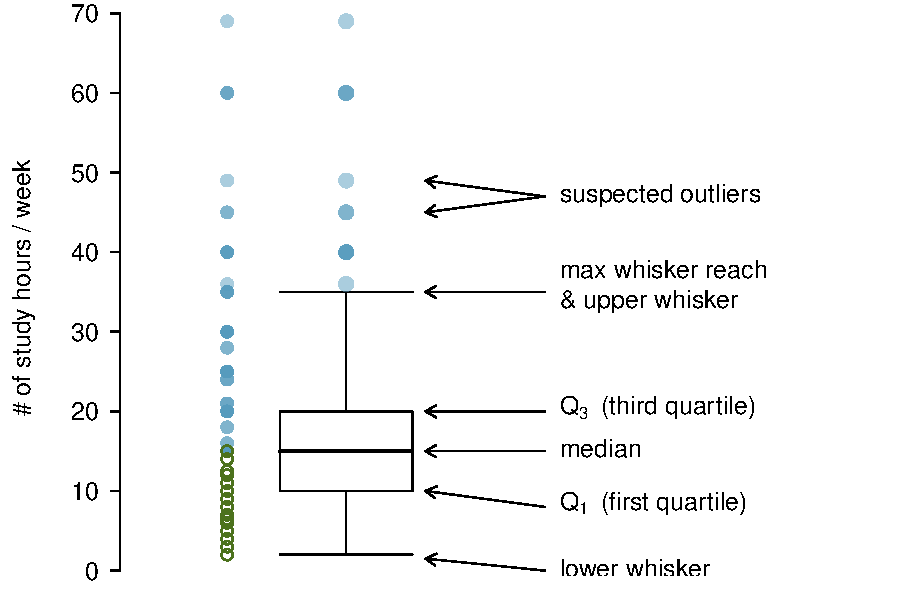
\includegraphics[width=0.95\textwidth]{\chpii@path/2-1_numerical_data/figures/study_hours/study_hours_box_layout}
\end{center}

\end{frame}

%%%%%%%%%%%%%%%%%%%%%%%%%%%%%%%%%%%%

\begin{frame}[fragile]
\frametitle{Whiskers and outliers}

\begin{itemize}

\item \hl{Whiskers} of a box plot can extend up to $1.5 \times IQR$ away from the quartiles.
\formula{
\vspace{-0.5cm}
\begin{align*} 
\text{max~upper~whisker~reach} &= Q3 + 1.5 \times IQR \\
\text{max~lower~whisker~reach} &= Q1 - 1.5 \times IQR
\end{align*}
}
\pause
\vspace{-0.5cm}
{\small
\begin{align*}
\text{IQR}&: 20 - 10 = 10 \\
\text{max~upper~whisker~reach}&= 20 + 1.5 \times 10 = 35 \\
\text{max~lower~whisker~reach}&= 10 - 1.5 \times 10 = -5
\end{align*}
}

\pause
\vspace{-0.25cm}
\item A potential \hl{outlier} is defined as an observation beyond the maximum reach of the whiskers. It is an observation that appears extreme relative to the rest of the data.

\end{itemize}

\end{frame}

%%%%%%%%%%%%%%%%%%%%%%%%%%%%%%%%%%%%

\begin{frame}
\frametitle{Outliers (cont.)}

\dq{Why is it important to look for outliers?}

\soln{
\onslide<2->{
\begin{itemize}
\item Identify extreme skew in the distribution.
\item Identify data collection and entry errors.
\item Provide insight into interesting features of the data.
\end{itemize}
}
}

\end{frame}

%%%%%%%%%%%%%%%%%%%%%%%%%%%%%%%%%%%%
\section{Edfinity Quiz}
%%%%%%%%%%%%%%%%%%%%%%%%%%%%%%%%%%%%

%%%%%%%%%%%%%%%%%%%%%%%%%%%%%%%%%%%%
\begin{frame}
\frametitle{How many outliers?}
\begin{center}
\begin{tikzpicture}
  % Image
  \node[anchor=south west,inner sep=0] (img) at (0,0) {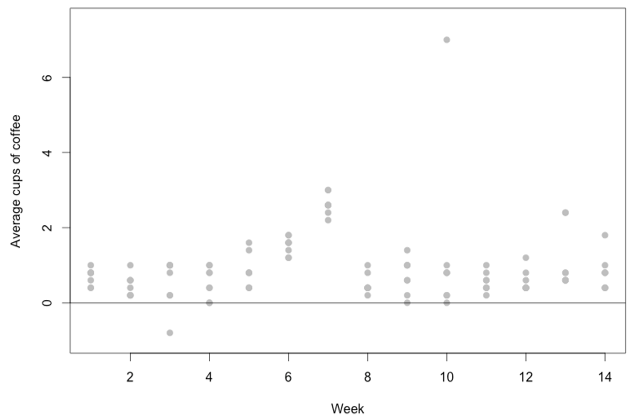
\includegraphics[width=0.95\textwidth]{avg_coffee.png}};
  % --- Stage 1: Median line ---
  \draw[red,thick] (-0.3,2.4) -- (0.0,2.4); % Median
  \node[anchor=east, text=red, font=\bfseries\small, visible on=<1>] at (-0.4,2.4) {Med};
  \pause
  % --- Stage 2: Q1 and Q3 lines ---
  \draw[red,thick] (-0.3,2.1) -- (0.0,2.1); % Q1
  \draw[red,thick] (-0.3,3.2) -- (0.0,3.2); % Q3
  \node[anchor=east, text=red, font=\bfseries\small, visible on=<2>] at (-0.4,2.1) {Q1};
  \node[anchor=east, text=red, font=\bfseries\small, visible on=<2>] at (-0.4,3.2) {Q2};
 \pause
  % --- Stage 3: Box verticals ---
  \draw[red,thick] (-0.3,2.1) -- (-0.3,3.2); % left vertical
  \draw[red,thick] (0.0,2.1) -- (0.0,3.2);  % right vertical
  \draw[red,thick, visible on=<3>] (-0.4,2.1) -- (-0.5,2.1) -- (-0.5,3.2) -- (-0.4,3.2);
  \node[anchor=east, text=red, font=\bfseries\small, visible on=<3>] at (-0.5,2.7) {IQR};
  \pause
  % --- Stage 4: Whiskers ---
  \draw[red,thick] (-0.3,0.6) -- (0.0,0.6); % Lower whisker
  \draw[red,thick] (-0.15,2.1) -- (-0.15,0.6); % Lower whisker
  \draw[red,thick] (-0.3,4.7) -- (0.0,4.7); % Upper whisker
  \draw[red,thick] (-0.15,3.2) -- (-0.15,4.7); % Upper whisker
  \pause
  % --- Outlier circles and Impossible label ---
  \draw[red,thick] (7.2,6.1) circle [radius=0.4]; % High outlier
  \pause
  \draw[red,thick] (2.7,1.4) circle [radius=0.4]; % Low outlier
  \node[anchor=west, text=red, font=\bfseries\large] at (3.2,1.4) {Impossible};
\end{tikzpicture}
\end{center}
\end{frame}
%%%%%%%%%%%%%%%%%%%%%%%%%%%%%%%%%%%%


%%%%%%%%%%%%%%%%%%%%%%%%%%%%%%%%%%%%
\section{Forum Brainstorm: Outliers}
%%%%%%%%%%%%%%%%%%%%%%%%%%%%%%%%%%%%

\begin{frame}
\frametitle{What to do with outliers?}
\begin{itemize}
\item \hl{Think:} 
\begin{itemize}
  \item What are some examples of outliers? 
  \item Are they errors or interesting features of the data?
  \item Under what circumstances would you keep or remove them?
\end{itemize}
\item \hl{Share:} Share an example with the class in the forum, and your thoughts on what do with it/why
\end{itemize}
\end{frame}

%%%%%%%%%%%%%%%%%%%%%%%%%%%%%%%%%%%%
\begin{frame}
\frametitle{What to do with outliers? It's a judgment call!}
\begin{itemize}
  \item Considerations:
  \begin{itemize}
    \item Are they consistent with the rest of the data, e.g. a "long tail"?
    \item Are they errors in data collection or entry, or data points from a different population?
    \item How will your analysis be affected by their presence?
  \end{itemize}
  \item Remove?
  \begin{itemize}
    \item If they are errors in data collection or entry
    \item If they are from a different population
  \end{itemize}
  \item Keep?
  \begin{itemize}
    \item Consider using robust statistics
    \item Consider using transformations e.g. to account for skewness
    \item (Advanced) Consider using a different model for your population
  \end{itemize}
  \item Look into them!
\end{itemize}
\end{frame}
%%%%%%%%%%%%%%%%%%%%%%%%%%%%%%%%%%%%

\subsection{Robust statistics}

%%%%%%%%%%%%%%%%%%%%%%%%%%%%%%%%%%%%

\begin{frame}
\frametitle{Extreme observations}

\dq{How would sample statistics such as mean, median, SD, and IQR of household income be affected if the largest value was replaced with \$10 million? What if the smallest value was replaced with \$10 million?}

\begin{center}
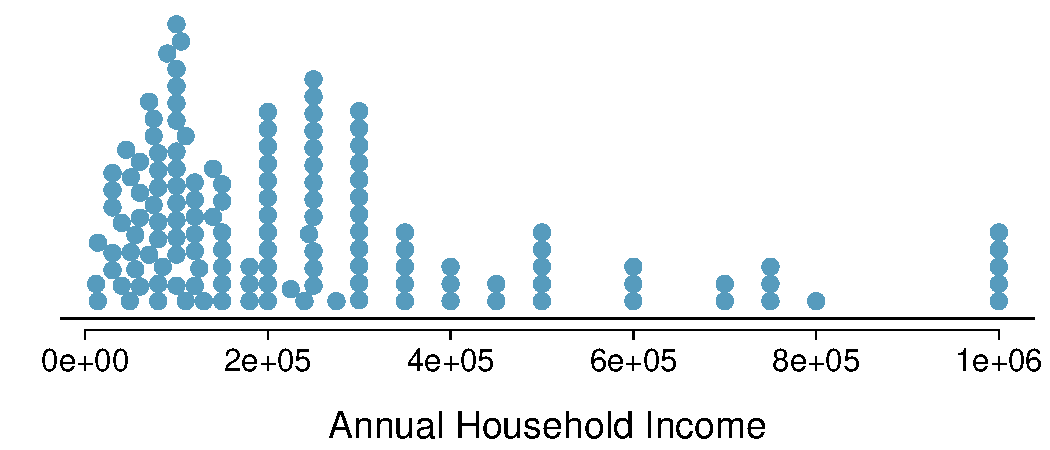
\includegraphics[width=\textwidth]{\chpii@path/2-1_numerical_data/figures/house_income/house_income_dot_stacked}
\end{center}

\end{frame}

%%%%%%%%%%%%%%%%%%%%%%%%%%%%%%%%%%%%

%%%%%%%%%%%%%%%%%%%%%%%%%%%%%%%%%%%
\section{Edfinity/applet: Robust statistics}
%%%%%%%%%%%%%%%%%%%%%%%%%%%%%%%%%%%

\begin{frame}
\frametitle{Robust statistics}

\begin{center}
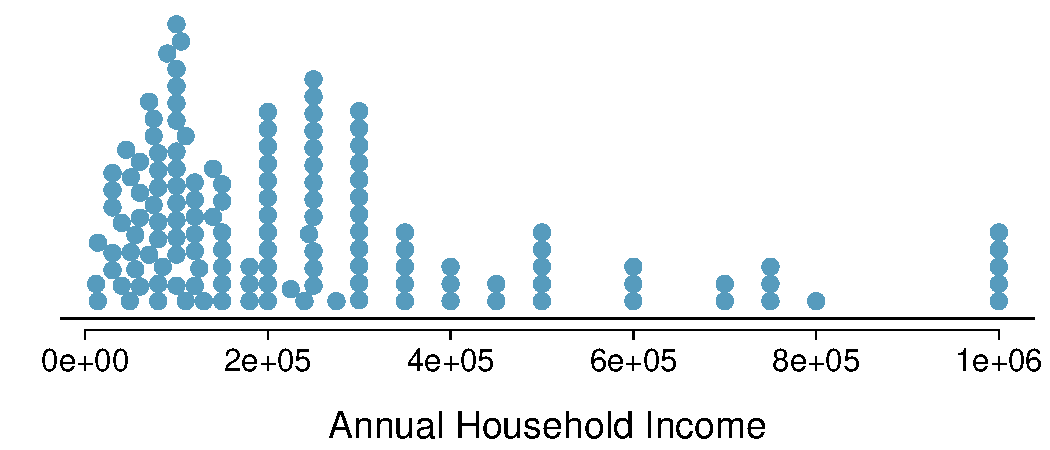
\includegraphics[width=\textwidth]{\chpii@path/2-1_numerical_data/figures/house_income/house_income_dot_stacked}
\end{center}

{\small
\begin{center}
\begin{tabular}{l c cc c cc}
  \hline
& \hspace{0mm} & \multicolumn{2}{c}{\bf robust} & \hspace{2mm} & \multicolumn{2}{c}{\bf not robust} \\
scenario && median & IQR && $\bar{x}$ & $s$ \\ 
  \hline
original data && 190K & 200K && 245K & 226K \\ 
move largest to \$10 million && 190K & 200K && 309K & 853K \\ 
move smallest to \$10 million && 200K & 200K && 316K & 854K \\ 
   \hline
\end{tabular}
\end{center}
}

\end{frame}

%%%%%%%%%%%%%%%%%%%%%%%%%%%%%%%%%%%%

\begin{frame}
\frametitle{Robust statistics}

Median and IQR are more robust to skewness and outliers than mean and SD. Therefore,

\begin{itemize}
\item for skewed distributions it is often more helpful to use median and IQR to describe the center and spread
\item for symmetric distributions it is often more helpful to use the mean and SD to describe the center and spread
\end{itemize}

$\:$ \\

\pause

\dq{If you would like to estimate the typical household income for a student, would you be more interested in the mean or median income?}

\soln{\pause{Median}}

\end{frame}

%%%%%%%%%%%%%%%%%%%%%%%%%%%%%%%%%%%%

\begin{frame}
\frametitle{Mean vs. median}

\begin{itemize}

\item If the distribution is symmetric, center is often defined as the mean: mean $\approx$ median

\begin{center}
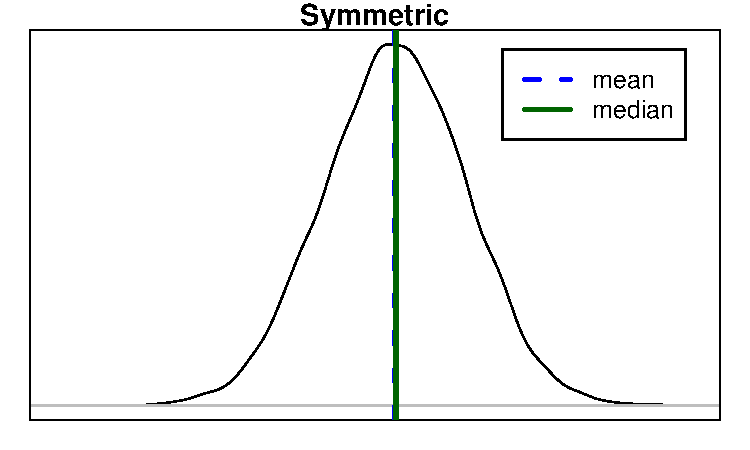
\includegraphics[width=0.33\textwidth]{\chpii@path/2-1_numerical_data/figures/mean_med/sym}
\end{center}

\item If the distribution is skewed or has extreme outliers, center is often defined as the median
\begin{itemize}
\item Right-skewed: mean $>$ median
\item Left-skewed: mean $<$ median \\
\end{itemize}

\end{itemize}

\begin{center}
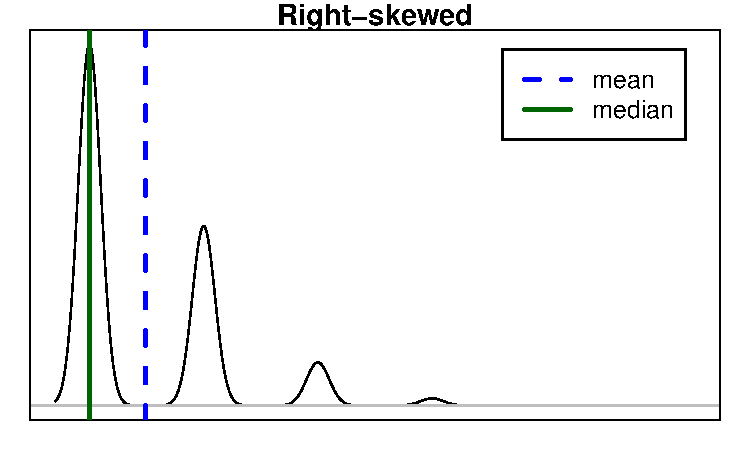
\includegraphics[width=0.33\textwidth]{\chpii@path/2-1_numerical_data/figures/mean_med/rs}
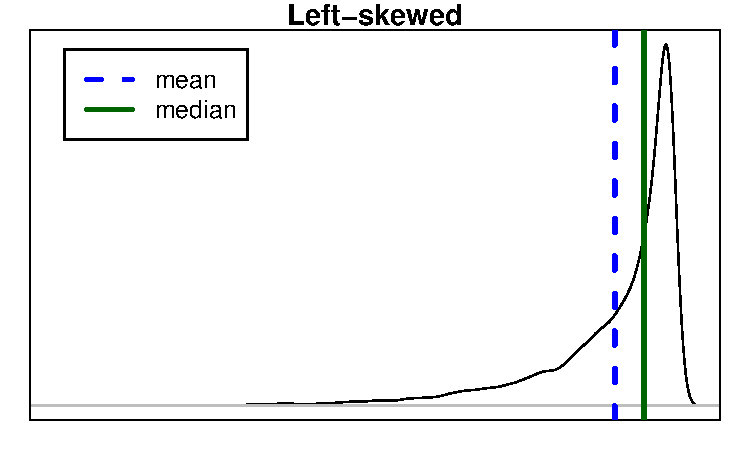
\includegraphics[width=0.33\textwidth]{\chpii@path/2-1_numerical_data/figures/mean_med/ls}\\
\end{center}

\end{frame}

%%%%%%%%%%%%%%%%%%%%%%%%%%%%%%%%%%%%%

% \begin{frame}
% \frametitle{Practice}

% \pq{{\small Which is most likely true for the distribution of percentage of time actually spent taking notes in class versus on Facebook, Twitter, etc.?}}

% \vspace{-0.5cm}

% \begin{columns}
% \column{0.7\textwidth}
% \begin{center}
% % 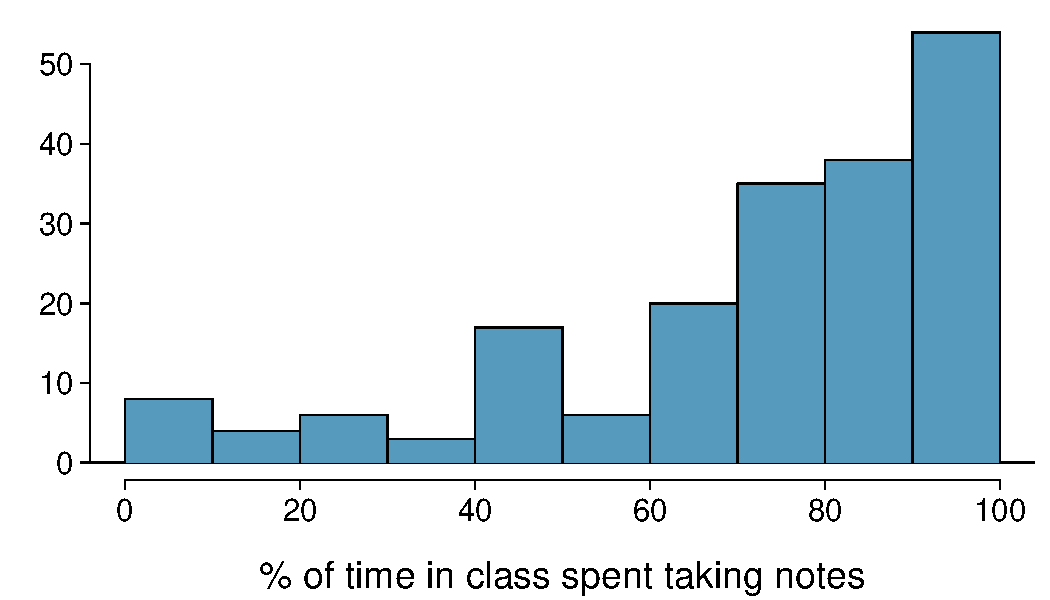
\includegraphics[width=0.9\textwidth]{\chpii@path/2-1_numerical_data/figures/notes_perc/notes_perc_hist}
% \end{center}
% \column{0.3\textwidth}
% $\:$ \\
% $\:$ \\
% \soln{\only<2>{\orange{median: 80\% \\ mean: 76\%}}}
% \end{columns}

% {\small
% \begin{multicols}{2}
% \begin{enumerate}[(a)]
% \item mean$>$ median
% \solnMult{mean $<$ median}
% \item mean $\approx$ median
% \item impossible to tell
% \end{enumerate}
% \end{multicols}
% }

% \end{frame}

%%%%%%%%%%%%%%%%%%%%%%%%%%%%%%%%%%%
\section{Edfinity: Mean/median}
%%%%%%%%%%%%%%%%%%%%%%%%%%%%%%%%%%%

%%%%%%%%%%%%%%%%%%%%%%%%%%%%%%%%%%%%%

\subsection{Transforming data}

%%%%%%%%%%%%%%%%%%%%%%%%%%%%%%%%%%%%

\begin{frame}
\frametitle{Extremely skewed data}

When data are extremely skewed, transforming them might make modeling easier. A common transformation is the \hl{log transformation}.

$\:$ \\
\pause
The histogram on the left shows the distribution of number of basketball games attended by students. The histogram on the right shows the distribution of log of number of games attended.

\begin{center}
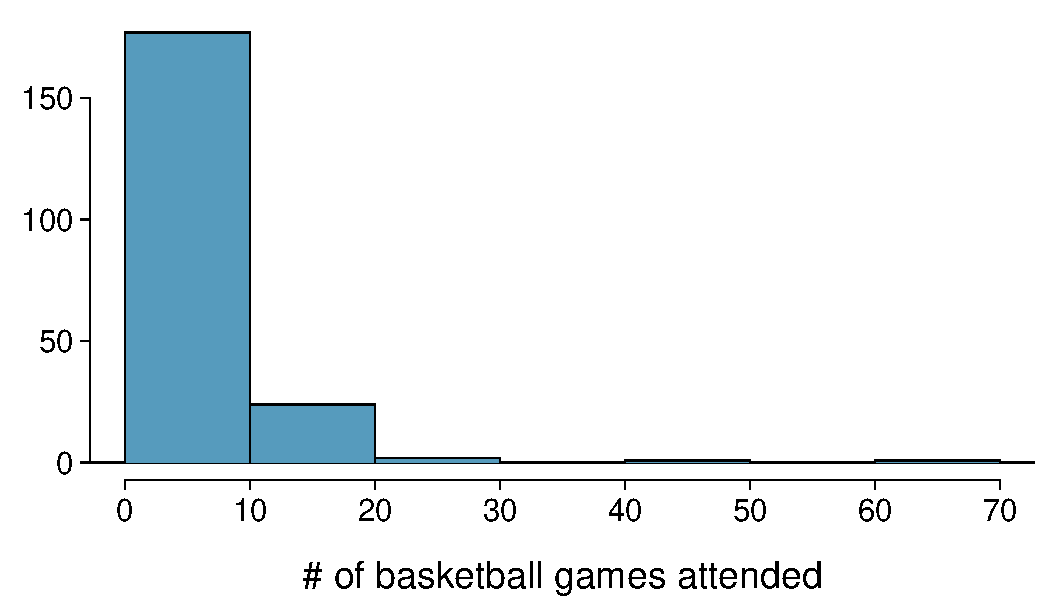
\includegraphics[width=0.45\textwidth]{\chpii@path/2-1_numerical_data/figures/basket_games/basket_games_hist}
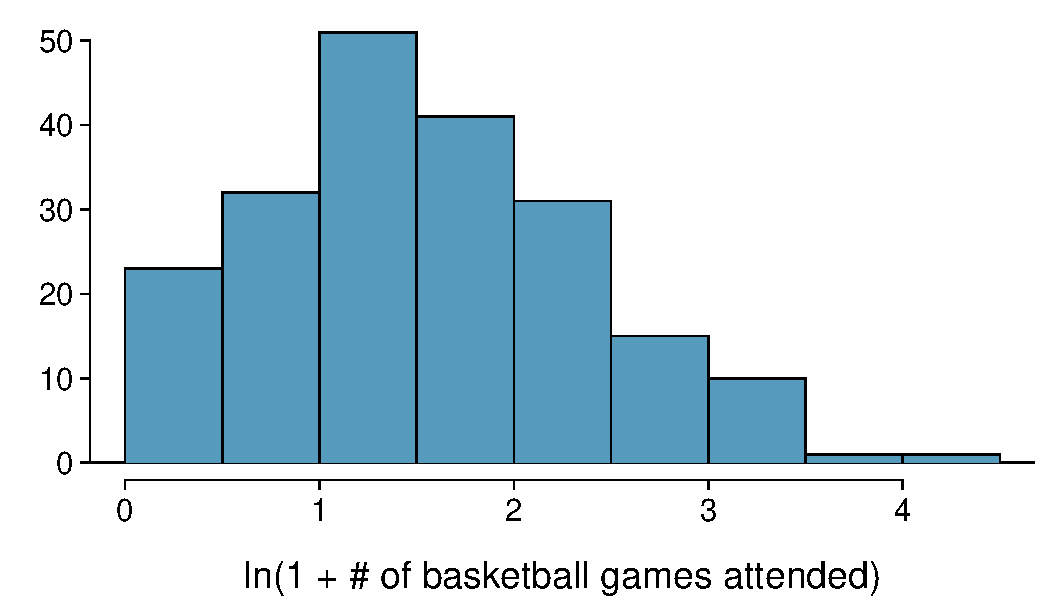
\includegraphics[width=0.45\textwidth]{\chpii@path/2-1_numerical_data/figures/basket_games/basket_games_hist_log}
\end{center}

\end{frame}

%%%%%%%%%%%%%%%%%%%%%%%%%%%%%%%%%%%%

\begin{frame}
\frametitle{Pros and cons of transformations}

\begin{itemize}

\item Skewed data are easier to model with when they are transformed because outliers tend to become far less prominent after an appropriate transformation. \\
$\:$ \\
\renewcommand{\arraystretch}{1.5}
\begin{tabular}{l r r r r }
\# of games		&  70 	& 50 		& 25 		 		& $\cdots$ \\
log(\# of games)	& 4.25	& 3.91 	& 3.22 	 	& $\cdots$
\end{tabular}

$\:$ \\

\item However, results of an analysis in log units of the measured variable might be difficult to interpret.

\end{itemize}

\pause

\dq{What other variables would you expect to be extremely skewed?}

\soln{\pause{Salary, housing prices, etc.}}

\end{frame}

%%%%%%%%%%%%%%%%%%%%%%%%%%%%%%%%%%%%

\subsection{Mapping data}

%%%%%%%%%%%%%%%%%%%%%%%%%%%%%%%%%%%%

\begin{frame}
\frametitle{Intensity maps}

\dq{What patterns are apparent in the change in population between 2000 and 2010?}

\begin{center}
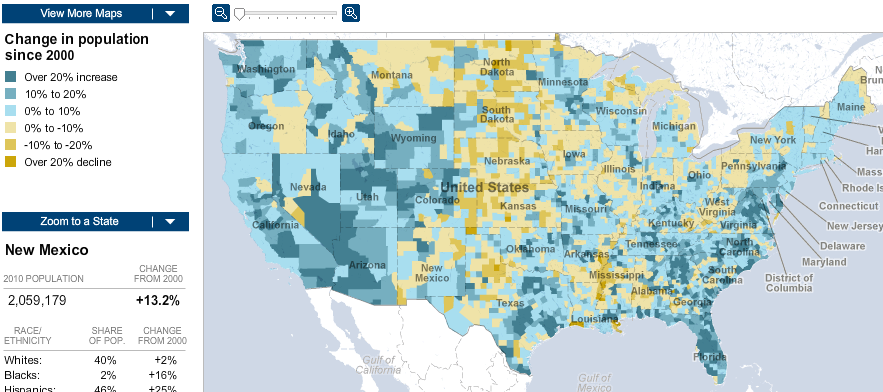
\includegraphics[width=0.95\textwidth]{\chpii@path/2-1_numerical_data/figures/change_in_pop_intensity}
\end{center}

\ct{\webURL{http://projects.nytimes.com/census/2010/map}}

\end{frame}


%%%%%%%%%%%%%%%%%%%%%%%%%%%%%%%%%%%%

%%%%%%%%%%%%%%%%%%%%%%%%%%%%%%%%%%%%

\section{Considering categorical data}

%%%%%%%%%%%%%%%%%%%%%%%%%%%%%%%%%%%%

\subsection{Contingency tables and bar plots}

%%%%%%%%%%%%%%%%%%%%%%%%%%%%%%%%%%%%

\begin{frame}
\frametitle{Contingency tables}

A table that summarizes data for two categorical variables is called a \hl{contingency table}.

$\:$ \\
\pause
The contingency table below shows the distribution of survival and ages of passengers on the Titanic.

\begin{center}
\begin{tabular}{l l cc r}
					               & 			 & \multicolumn{2}{c}{{Survival}} \\
  \cline{3-4}
					               &			 & Died	 & Survived	& Total \\ 
  \cline{2-5}
\multirow{2}{*}{{Age}}& Adult & 1438  & 654 	  	& 2092 \\ 
  					             & Child & 52 	 & 57	 	    & 109\\ 
  \cline{2-5}
  					             & Total & 1490  & 711	    &  2201 \\
  \cline{2-5}
\end{tabular}
\end{center}
\end{frame}

%%%%%%%%%%%%%%%%%%%%%%%%%%%%%%%%%%%%

\begin{frame}
\frametitle{Bar plots}

A \hl{bar plot} is a common way to display a single categorical variable. A bar plot where proportions instead of frequencies are shown is called a \hl{relative frequency bar plot}.

\begin{center}
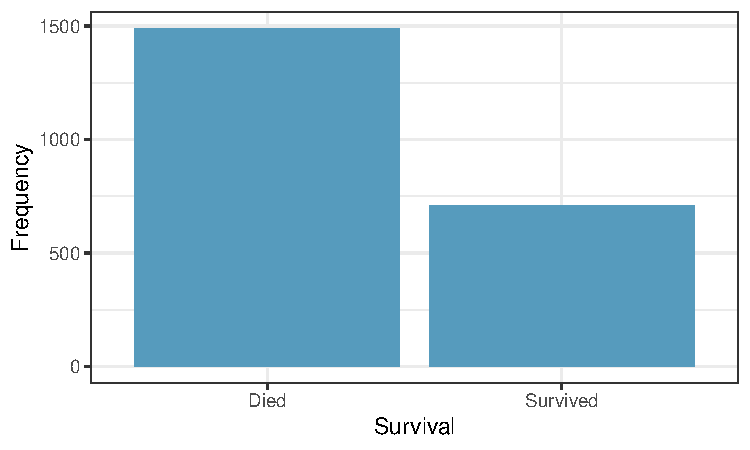
\includegraphics[width=0.45\textwidth]{\chpii@path/2-2_categorical_data/figures/titanic_age_survival/titanic_bar}
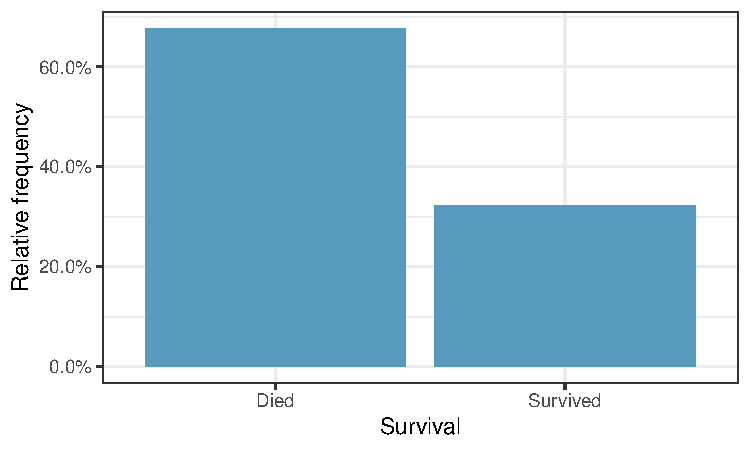
\includegraphics[width=0.45\textwidth]{\chpii@path/2-2_categorical_data/figures/titanic_age_survival/titanic_rel_bar}
\end{center}

\pause

\dq{How are bar plots different than histograms?}

\soln{\pause{{\tiny Bar plots are used for displaying distributions of categorical variables,  histograms are used for numerical variables. The x-axis in a histogram is a number line,  hence the order of the bars cannot be changed. In a bar plot, the categories can be listed in any order (though some orderings make more sense than others, especially for ordinal variables.)}}}

\end{frame}

%%%%%%%%%%%%%%%%%%%%%%%%%%%%%%%%%%%%

\subsection{Row and column proportions}

%%%%%%%%%%%%%%%%%%%%%%%%%%%%%%%%%%%%

\begin{frame}
\frametitle{Choosing the appropriate proportion}

\dq{Does there appear to be a relationship between age and survival for passengers on the Titanic?}

\begin{center}
\begin{tabular}{l l cc r}
					               & 			 & \multicolumn{2}{c}{{Survival}} \\
  \cline{3-4}
					               &			 & Died	 & Survived	& Total \\ 
  \cline{2-5}
\multirow{2}{*}{{Age}}& Adult & 1438  & 654 	  	& 2092 \\ 
  					             & Child & 52 	 & 57	 	    & 109\\ 
  \cline{2-5}
  					             & Total & 1490  & 711	    &  2201 \\
  \cline{2-5}
\end{tabular}
\end{center}

\pause

To answer this question we examine the row proportions: 

\pause

\begin{itemize}

\item \% Adults who survived: 654 / 2092 $\approx 0.31$ \\

\pause

\item \% Children who survived: 57 / 109 $\approx 0.52$ \\

\end{itemize}

\end{frame}

%%%%%%%%%%%%%%%%%%%%%%%%%%%%%%%%%%%%

\subsection{Using a bar plot with two variables}

%%%%%%%%%%%%%%%%%%%%%%%%%%%%%%%%%%%%

\begin{frame}
\frametitle{Bar plots with two variables}

\begin{itemize}

\item \hl{Stacked bar plot:} Graphical display of contingency table information,
for counts.

\item \hl{Side-by-side bar plot:} Displays the same information by placing bars 
next to, instead of on top of, each other.

\item \hl{Standardized stacked bar plot}: Graphical display of contingency table 
information, for proportions.

\end{itemize}

\end{frame}

%%%%%%%%%%%%%%%%%%%%%%%%%%%%%%%%%%%%

\begin{frame}

\dq{What are the differences between the three visualizations shown below?}

\begin{center}
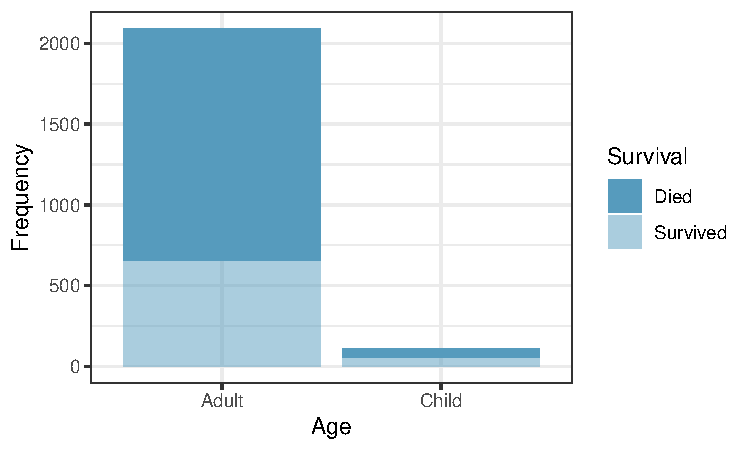
\includegraphics[width=0.45\textwidth]{\chpii@path/2-2_categorical_data/figures/titanic_age_survival/titanic_seg_bar}
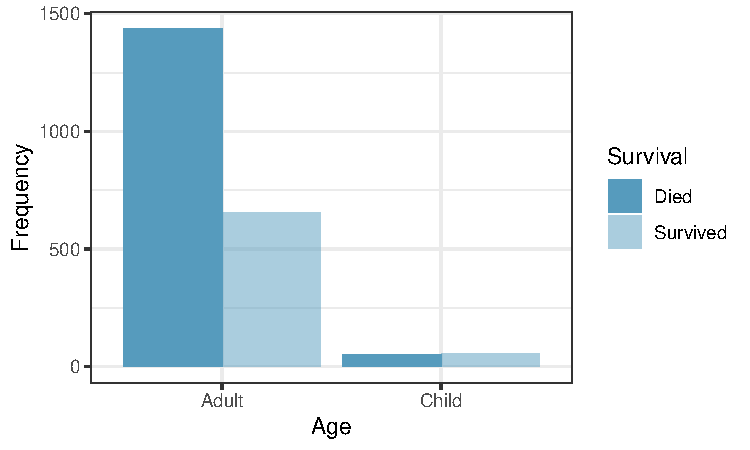
\includegraphics[width=0.45\textwidth]{\chpii@path/2-2_categorical_data/figures/titanic_age_survival/titanic_seg_bar_dodge} \\
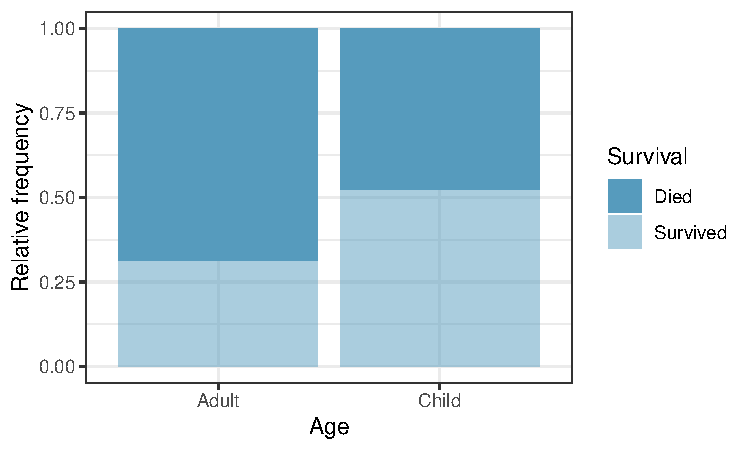
\includegraphics[width=0.45\textwidth]{\chpii@path/2-2_categorical_data/figures/titanic_age_survival/titanic_rel_seg_bar}
\end{center}

\end{frame}

%%%%%%%%%%%%%%%%%%%%%%%%%%%%%%%%%%%%

\subsection{Mosaic plots}

%%%%%%%%%%%%%%%%%%%%%%%%%%%%%%%%%%%%

\begin{frame}
\frametitle{Mosaic plots}

\dq{What is the difference between the two visualizations shown below?}

\begin{center}
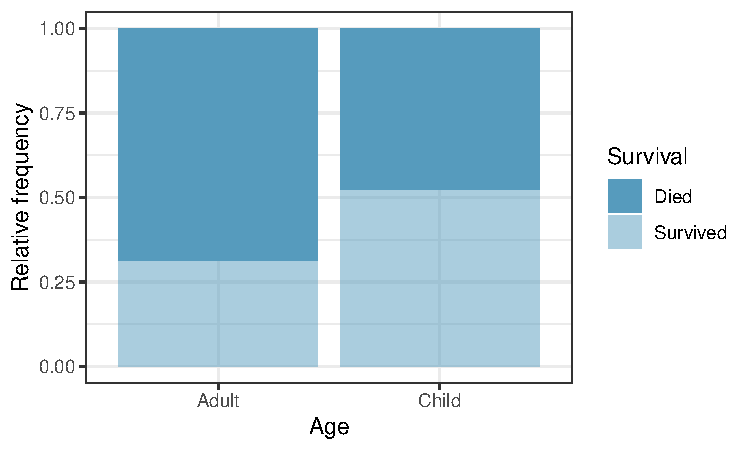
\includegraphics[width=0.45\textwidth]{\chpii@path/2-2_categorical_data/figures/titanic_age_survival/titanic_rel_seg_bar}
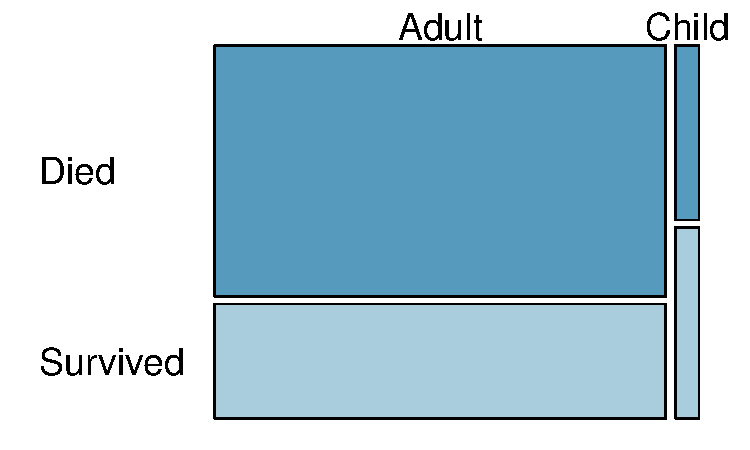
\includegraphics[width=0.45\textwidth]{\chpii@path/2-2_categorical_data/figures/titanic_age_survival/titanic_mosaic}
\end{center}

\end{frame}

%%%%%%%%%%%%%%%%%%%%%%%%%%%%%%%%%%%%

\subsection{Pie charts}

%%%%%%%%%%%%%%%%%%%%%%%%%%%%%%%%%%%%

\begin{frame}
\frametitle{Pie charts}

\dq{Can you tell which order encompasses the lowest percentage of mammal species?}

\vspace{-0.5cm}

\begin{center}
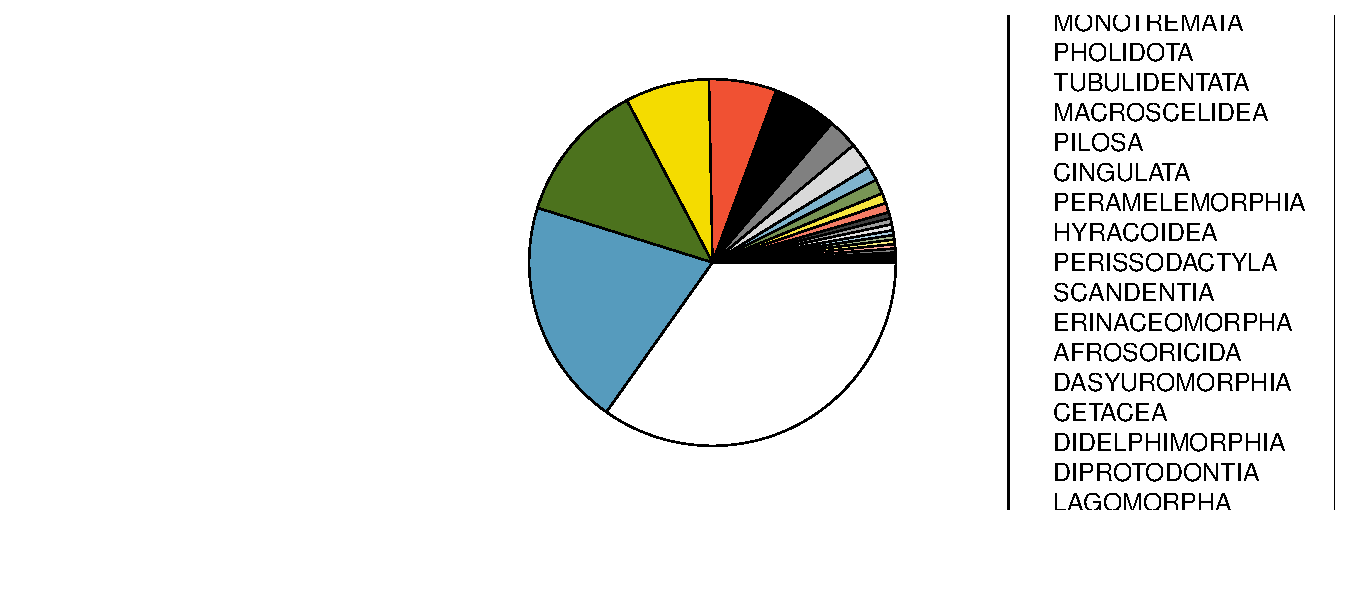
\includegraphics[width=0.4\textwidth]{\chpii@path/2-2_categorical_data/figures/mammal_pie_chart/mammal_pie_chart}
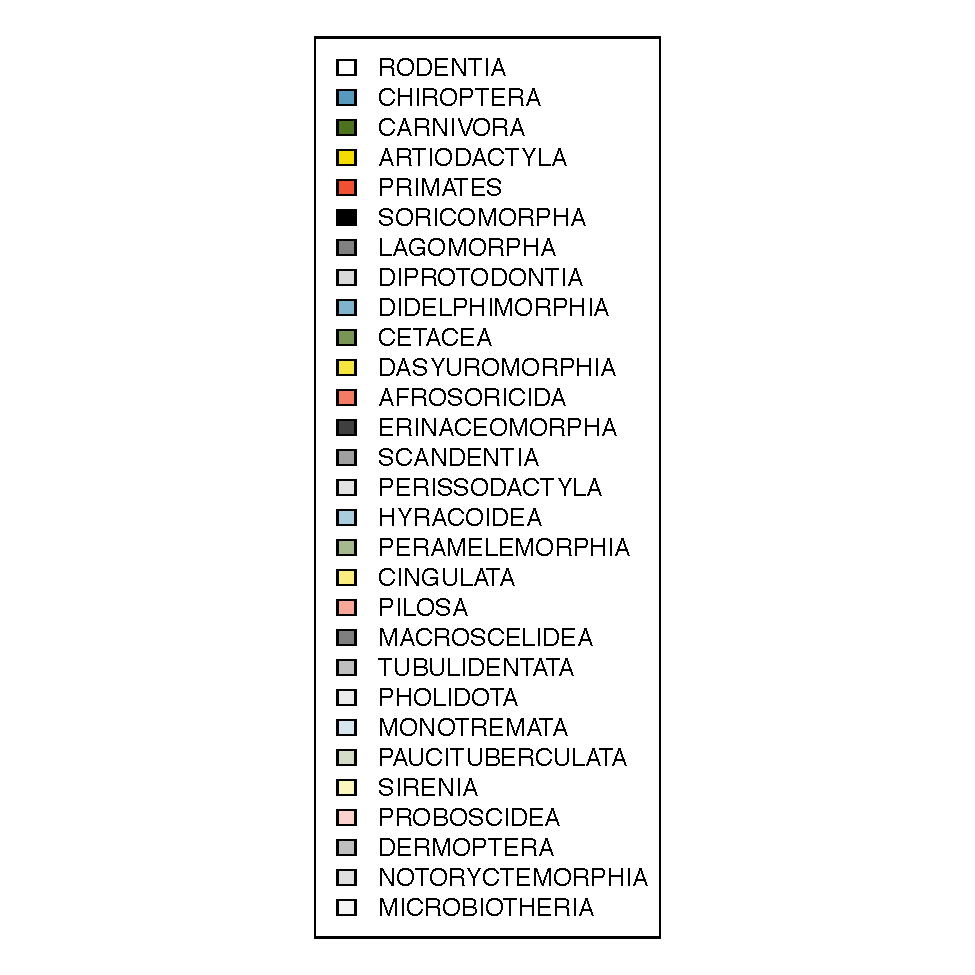
\includegraphics[width=0.2\textwidth]{\chpii@path/2-2_categorical_data/figures/mammal_pie_chart/mammal_pie_chart_legend}
\end{center}

\ct{Data from \webURL{http://www.bucknell.edu/msw3}.}

\end{frame}


%%%%%%%%%%%%%%%%%%%%%%%%%%%%%%%%%%%%

\subsection{Comparing numerical data across groups}

%%%%%%%%%%%%%%%%%%%%%%%%%%%%%%%%%%%%

\begin{frame}
\frametitle{Side-by-side box plots}

\dq{Does there appear to be a relationship between class year and number of clubs students are in?}

\begin{center}
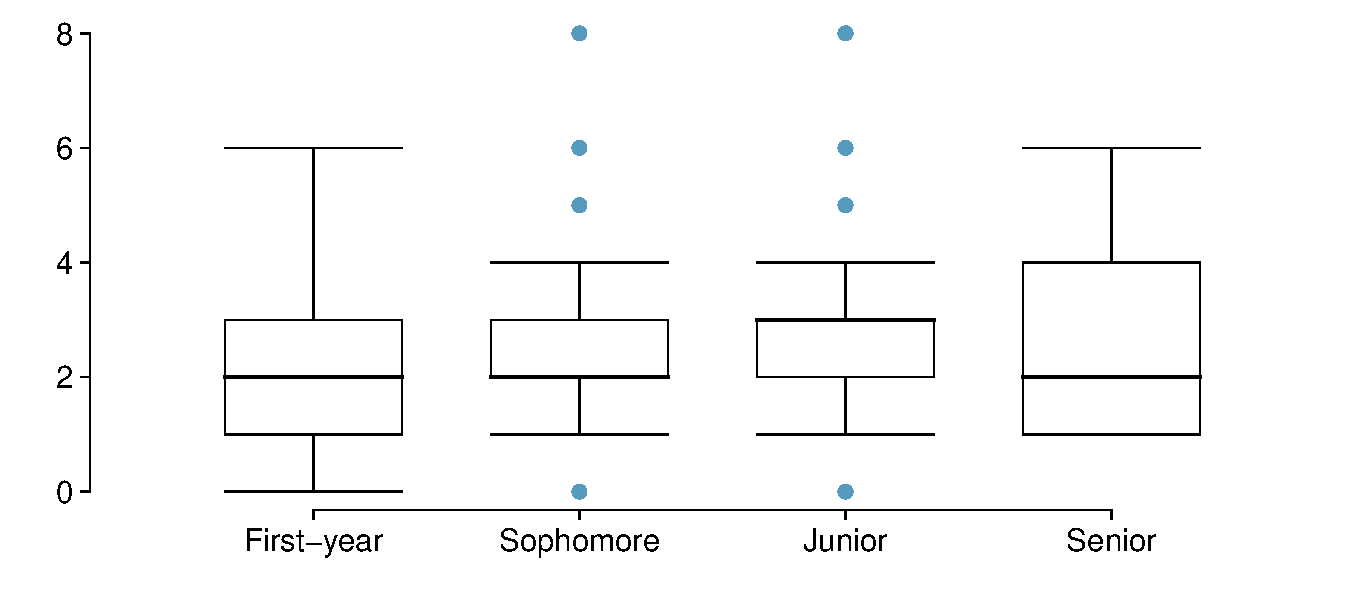
\includegraphics[width=\textwidth]{\chpii@path/2-2_categorical_data/figures/year_clubs/year_clubs}
\end{center}

\end{frame}

%%%%%%%%%%%%%%%%%%%%%%%%%%%%%%%%%%%%

\section{Edfinity Quiz}

%%%%%%%%%%%%%%%%%%%%%%%%%%%%%%%%%%%%

%%%%%%%%%%%%%%%%%%%%%%%%%%%%%%%%%%%%
% End document
%%%%%%%%%%%%%%%%%%%%%%%%%%%%%%%%%%%%

\end{document}